\documentclass{achemso}
%\documentclass[prb,preprint,12pt,superscriptaddress,unsortedaddress,floatfix,bibnotes,nofootinbib,unsortedaddress]{revtex4}


%%%%%%%%%%%%%%%%%%%%%%%%%%%%%%%%%%%%%%%%%%%%%%%%%%%%%%%%%%%%%%%%%%%%%
%% If issues arise when submitting your manuscript, you may want to
%% un-comment the next line.  This provides information on the
%% version of every file you have used.
%%%%%%%%%%%%%%%%%%%%%%%%%%%%%%%%%%%%%%%%%%%%%%%%%%%%%%%%%%%%%%%%%%%%%
\usepackage{natbib}
\usepackage{lineno}
\linenumbers
\usepackage{arydshln}
\usepackage{bibentry}
\usepackage{verbatim}
\usepackage{epsf}
\usepackage{color}
\usepackage{mathtools}
\usepackage{amssymb}
\usepackage{bm}% bold math
\usepackage{graphicx}
\usepackage{epstopdf}
\epstopdfsetup{update} % only regenerate pdf files when eps file is newer
\renewcommand{\thefootnote}{\fnsymbol{footnote}}
\renewcommand{\eqref}[1]{(\ref{#1})}
\newcommand{\ds}{\displaystyle}
\def\ii{{\'\i} }
\newcommand{\red}[1]{{\color{red} #1}}
\newcommand{\3}{$_{3}$}
\newcommand{\cm}{cm$^{-1}$}
\newcommand{\lnr}{^{\ell}}
%\newcommand{\mathbf}[1]{{\mathbf #1}}
\newcommand{\abinitio}{\textit{ab initio}}
\newcommand{\Abinitio}{\textit{Ab initio}}
\newcommand{\citings}[6]{#1, \textit{#2}  \textbf{#6}, \textit{#3}, #4.} %
\newcommand{\ftnm}[1]{\footnotemark[#1]}
\newcommand{\onlinecite}[1]{\citenum{#1}}
\newcommand{\citingsjcp}[6]{#1, {#2} #3, #4 (#6).}         % JCP-style
\newcommand{\p}{^\prime}
\newcommand{\pp}{^{\prime\prime}}
\newcommand{\Dh}{{\itshape\bfseries D}$_{3{\rm h}}$}
\font\bmit=cmmib10
%\def\bm{\mu}{\hbox{\bmit\char'26}}
\def\bomega{\hbox{\bmit\char'41}}
\def\bepsilon{\hbox{\bmit\char'17}}
\newcommand{\ai}{\textit{ab initio}}
\mciteErrorOnUnknownfalse
%------
% Title
%------

\title[Line List for Methyl Radical]{ A variationally computed IR line list for the methyl radical CH\3}

%--------
% Authors
%--------

%---------------------
\author{Ahmad Y. Adam}
%---------------------
\affiliation[Bergische Universit{\"a}t]{Fakult{\"a}t f{\"u}r Mathematik und Naturwissenschaften, Physikalische
und Theoretische Chemie, Bergische Universit{\"a}t Wuppertal, D--42097 Wuppertal, Germany}
%---------------------------
\author{Andrey Yachmenev}
%---------------------------
\affiliation[DESY and Universit{\"a}t Hamburg]{Center for Free-Electron Laser Science, Deutsches Elektronen-Synchrotron DESY, Notkestra{\ss}e 85, D-22607 Hamburg, Germany,
The Hamburg Center for Ultrafast Imaging, Universit{\"a}t Hamburg, Luruper Chaussee 149, D-22761 Hamburg, Germany}
%---------------------------
\author{Sergei N. Yurchenko}
%---------------------------
\affiliation[University College London]{Department of Physics and Astronomy, University College London,
Gower Street, London WC1E 6BT, United Kingdom}
%------------------
\author{Per Jensen}
%------------------
%\altaffiliation{To whom correspondence should be addressed. EMail: Per Jensen jensen@uni-wuppertal.de}
\affiliation[Bergische Universit{\"a}t]{Fakult{\"a}t f{\"u}r Mathematik und Naturwissenschaften, Physikalische
und Theoretische Chemie, Bergische Universit{\"a}t Wuppertal, D--42097 Wuppertal, Germany}
\email{jensen@uni-wuppertal.de}

%-----
% Date
%-----

\date{\today}

%---------------
\begin{document}
%---------------

%---------------
\begin{abstract}
%---------------
We present the first variational calculation of a hot temperature \textit{ab initio} line list for
the CH$_3$  radical. It is based on a high level {\it ab initio} potential energy surface and dipole
moment surface of CH$_3$ in the ground electronic state. The ro-vibrational energy levels and Einstein
 $A$ coefficients were calculated using the general-molecule variational approach implemented in the
computer program TROVE. Vibrational energies and vibrational intensities are found to be in  very good
agreement with the available experimental data. The line list comprises 9,127,123 ro-vibrational states ($J\le 40$) and 2,058,655,166 transitions covering the wavenumber range up to 10000~cm$^{-1}$ and should be suitable for temperatures up to $T= 1500$~K.

%-------------
\end{abstract}
%-------------

%------------------------------------------
\section{Introduction} \label{sec:intro}
%------------------------------------------

The methyl radical is one of the most important free radicals and plays a central role in hydrocarbon
combustion processes\cite{comb90} in atmospheric chemistry\cite{atmo88}, in the chemistry of
semiconductor production\cite{semi87}, in the chemical vapor deposition of diamond\cite{diamond91},
and in many chemical processes of current industrial and environmental interest. It is also present
in exo-planetary atmospheres \cite{astro02}, in the atmospheres of Saturn\cite{astro98} and Neptune\cite{astro99},
and in the interstellar medium,\cite{astro00} where it is thought to be one of the most abundant
free radicals.\cite{astro02} Because of its central role in this variety
of situations, its structural and spectroscopic parameters have been the subject of numerous studies.
A number of different spectroscopic techniques have been used to determine its absolute concentration
in the gas phase, including UV/visible\cite{xelec03}, infrared\cite{nu2_72}, and Raman spectroscopies
\cite{nu1_84,nu1_88,nu1_92,nu1_94,nu1_96,dnu1_89a,dnu1_89b}.  In addition, CH$_3$ is an example of
a molecule with large vibrational contribution to the hyperfine coupling constant, accounting for up
to about 41\%\ of the total value (see Ref.~\citenum{aa15} and references therein).

Owing to the importance of CH$_3$ in various contexts, in particular in astrophysics and -chemistry,
its concentrations or column densities in remote environments such as interstellar space, the terrestrial
atmosphere, exo-planetary atmospheres, and the outer layers of cool stars are of interest and it is
desirable to determine these by remote-sensing spectroscopic methods. A prerequisite for such determinations
is the knowledge of the transition moments for the observed transitions, and these must often be obtained
in theoretical calculations as done, for example, in the ExoMol project\cite{jt528,exomol} by Yurchenko and
co-workers.\cite{jt564,nh3_09,jt571,jt592,jt580,jt641,jt597,jt612,jt701,jt620,jt638,jtlinTROVE,jt729}
This project aims at providing theoretically computed transition moments and simulated spectra for (small
to medium-sized) general polyatomic molecules of astrophysical and/or -chemical interest.

At equilibrium, the three protons of electronic-ground-state $\tilde{X}$~$^2A''_2$
CH$_3$ form an equilateral triangle with the C nucleus at the centre-of-mass of the planar structure
with {\itshape\bfseries D}$_{3{\rm h}}$ point group symmetry (see Table~A-10 of Ref.\citenum{mss}).
There is no permanent dipole moment, and so the pure rotational transitions are dipole forbidden and
very weak. Also, the planar ground-state equilibrium structure precludes most one-photon transitions
to excited electronic states.\cite{xelec83} Owing to the extremely weak rotational spectrum, determinations
of concentrations and column densities for CH$_3$ must be made with rovibrational transitions in the
infrared region. The most suitable transitions are those in the intense $\nu_2$ fundamental band at
606~cm$^{-1}$ (where $\nu_2$ is the out-of-plane bending mode). This band provides convenient transitions
for concentration measurements and  has been used extensively for this purpose\cite{mu2_83,mu2_89,mu2_05,mu2_08}.
As mentioned above, the corresponding transition moments must be known in order that concentrations
can be determined, and the present work can be viewed as a first step towards providing extensive
catalogues of theoretical transition moments for CH$_3$, so-called line lists, of use in astrophysical
studies. In the present work we apply a high level \ai\ potential energy surface, refined by means
of experimental spectroscopic data, and \ai\ dipole moment surfaces to compute, with the TROVE program,
\cite{trove05,trove07,trove15,trove17a} sufficient energies and transition moments for generating
a hot ($T=1500$~K) IR line list for CH$_3$.

%----------------------------------------------
\section{Potential energy and dipole moment}
%----------------------------------------------

\subsection{Potential energy surface}\label{sec:PES}

The potential energy surface (PES) employed for the electronic ground state of CH\3\ in the present
work is based on the \ai\ surface reported in Ref.\citenum{aa15}, which we denote as PES-1. The PES-1
electronic energies were computed on a grid of 24\,000 symmetry-unique molecular geometries employing
the open-shell RCCSD(T)-F12b~\cite{adler07,adler09} level of theory (explicitly correlated F12 restricted
coupled cluster included single and double excitations with a noniterative correction for triples) and the
F12-optimized correlation consistent polarized valence basis set cc-pVQZ-F12.\cite{peterson08} In correlated
calculations the carbon inner-shell electron pair was treated as frozen core. The analytical representation
for the PES was obtained in a least-squares fitting procedure using the functional form from {Lin {\it et al.}
\cite{nh3_02}}:

%%%%%%%%%%%%%%%%%%%
\begin{eqnarray}
%\lefteqn{%
V(\xi_1,\xi_2,\xi_3,\xi_{4a},\xi_{4b};{\sin\bar \rho}) \,
    &=&  V_{\rm e} +  V_0({\sin\bar \rho}) + \sum_j \, F_j({\sin\bar \rho}) \, \xi_j
\nonumber \\
& + &
       \sum_{j \leqslant  k} \, F_{jk}({\sin\bar \rho}) \, \xi_j \, \xi_k
%
       +  \sum_{j \leqslant k \leqslant l} \, F_{jkl}({\sin\bar \rho}) \,\xi_j \, \xi_k \, \xi_l
\nonumber \\
       &+ & \sum_{j \leqslant k \leqslant l \leqslant m} \, F_{jklm}({\sin\bar \rho}) \, \xi_j \, \xi_k \,
        \xi_l \, \xi_m + \dots;
\label{e:PEF:morbid}
\end{eqnarray}
%%%%%%%%%%%%%%%
this function is expressed in terms of the stretching variables
\begin{equation}
\xi_k =
1 - \exp\left[ -a ( r_k - r_{\rm e}) \right], \;\; k=1,2,3,
\end{equation}
where
 $r_k$ is the instantaneous value of the distance
between the C nucleus
 and the proton H$_k$
labeled $k$ $=$ 1, 2, or 3;
$r_{\rm e}$ is the common equilibrium value of
the three $r_k$ bond lengths,
and $a$ is a Morse parameter.
Furthermore,
the symmetrized bending variables
$( \xi_{4a}, \xi_{4b} )$ are defined as
%%%%%%%%%%%%%%%%%%%%%
\begin{equation}
\label{S4a4b}
\left( \xi_{4a}, \xi_{4b} \right) =
\left(
  \frac{1}{\sqrt{6}} [2 \, \alpha_{1} - \alpha_{2} - \alpha_{3} ],
 \frac{1}{\sqrt{2}} [\alpha_{2} - \alpha_{3} ]
\right)
\end{equation}
with
$\alpha_i$ as      the bond angle $\angle$(H$_j$XH$_k$) where $(i,j,k)$ is a
permutation of the numbers (1,2,3).
%%%%%%%%%%%%%%%%%%%%%
Finally,
the variable
%%%%%%%%%%%%%%%%%%%%%
\begin{equation}
\label{e:sin:brho} \sin {\bar \rho} \, = \, \frac{2}{\sqrt{3}} \,
\sin [
   (\alpha_1 + \alpha_2 + \alpha_3) /6] \hbox{}
\end{equation}
%%%%%%%%%%%%%%%%
describes  the out-of-plane bending.
At the planar equilibrium configuration, we have
   $\alpha_1 + \alpha_2 + \alpha_3$ $=$ 360$^\circ$ and so
$\sin {\bar \rho}$ $=$
$\sin {\bar \rho}_{\rm e}$ $=$ 1.
%%%%%%%%%%%%%%%%%%%% NEW %%%%%%%%%%%%%%%%%%%%%%%%%%%%%
The functions $V_0({\sin\bar \rho})$ and  $F_{jk\dots}({\sin\bar \rho})$
in Eq.~\eqref{e:PEF:morbid} are defined as
%%%%%%%%%%%%%%%%%%%%
\begin{eqnarray}
\label{V0}
   V_0({\sin\bar \rho}) &=& \sum_{s=1}^{4} \, f_0^{(s)} \, (1           - \sin {\bar \rho})^s \hbox{,} \\
\label{Ffunction}
  F_{jk\dots}({\sin\bar \rho}) &=& \sum_{s=0}^{N}\, f_{jk\dots}^{(s)} \, (1 - \sin {\bar \rho})^s \hbox{,}
\end{eqnarray}
%%%%%%%%%%%%%%%%%%%%
%%%%%%%%%%%%%%%%%%%% NEW %%%%%%%%%%%%%%%%%%%%%%%%%%%%%
where
the quantities  $f_0^{(s)}$ and $f_{jk\dots}^{(s)}$ in
Eqs.~(\ref{V0}) and~(\ref{Ffunction}) are expansion coefficients.
 The optimized values of the parameters
$a$,
$r_{\rm e}$,
 $f_0^{(s)}$, and $f_{jk\dots}^{(s)}$
are given in the supplementary material to
 Ref.~\citenum{aa15} together with
 Fortran~90 routine for calculating PES values.

The analytical form of PES-1\cite{aa15}
is given in terms of
 the \abinitio\ cc-pVQZ-F12 values of the
equilibrium structural parameters,
$r_{\rm e} = 1.0774$~\AA\ and $\alpha_{\rm e}=
120.0^\circ$,\cite{aa15}
for the electronic ground state of CH\3. In the present work, we optimized
the values
 $r_{\rm e}$ and $\alpha_{\rm_e}$ in a least-squares fitting to experimentally derived
to rotational energy spacings within
 the vibrational states of CH\3.
The fitting produced the values of
$r_{\rm e} = 1.0763$~\AA\  and
$\alpha_{\rm e} = 120.0 $.
We adopt these optimized values of the equilibrium structural parameters.
All results presented in the remainder of the present work are based on
the analytical potential energy function called PES-2, obtained from PES-1\cite{aa15}
by replacing the
 \abinitio\ cc-pVQZ-F12 values of
$r_{\rm e}$ and $\alpha_{\rm e}$ by
the adjusted values given here. The remaining PES-2 parameter values are identical to
those of PES-1 and can be obtained from
the supplementary material to Ref.~\citenum{aa15}.

\subsection{Dipole moment surface}\label{sec:DMS}

The dipole moment surface (DMS) for the electronic ground state of CH$_3$ was computed using the
MOLPRO\cite{molpro12}  program package. Frozen-core calculations were carried out for 19\,361
symmetry-unique geometries (15\,600 below 30\,000~\cm) using the spin-restricted open-shell coupled
cluster theory RCCSD(T)~\cite{watts} and the augmented correlation consistent valence basis set
aug-cc-pVTZ~\cite{dunning,kendall}, employing the two-point stencil central
finite differences with the electric field strength of 0.002~a.u.


We employ the so-called symmetrized molecular-bond (SMB) representation\cite{nh3_09}
[which is an extension of the
 molecular-bond (MB)
representation~\cite{nh3_05}]
to formulate analytical functions describing the molecular dipole moment
components.
The SMB representation makes use of
the projections
 $ \bar{\bm{\mu}} \cdot \mathbf{e}_k $
of the dipole moment on the molecular
bonds, where
  $\mathbf{e}_k$ is  the unit vector along the
C--H$_k$ bond,
%sy line removed
\begin{equation}\label{e:e:r}
   \mathbf{e}_k = \frac{\mathbf{r}_k-\mathbf{r}_4}{|\mathbf{r}_k-\mathbf{r}_4|}
\end{equation}
%sy line removed
with $\mathbf{r}_k$, $k$ $=$ 1, 2, 3, as the position vector of proton $k$ and
$\mathbf{r}_4$ as the position vector of the C nucleus.

We form                                           symmetry-adapted
linear combinations of the MB projections $ \bar{\bm{\mu}} \cdot
\mathbf{e}_j $:
%%%%%%%%%%%%%%%%%%%%%%%%%%%%%%%%%%%%%%%%
\begin{eqnarray}
\label{e:mu:A}
  \bar\mu_{A_2\pp}^{\rm SMB}&=& \left( \bar{\bm{\mu}} \cdot \mathbf{e}_{\rm N} \right) \\
\label{e:mu:Ea}
  \bar\mu_{E_a\p}^{\rm SMB} &=& \frac{1}{\sqrt{6}} \left[ 2 \left( \bar{\bm{\mu}} \cdot \mathbf{e}_1 \right) - \left( \bar{\bm{\mu}} \cdot \mathbf{e}_2 \right) - \left( \bar{\bm{\mu}} \cdot \mathbf{e}_3 \right) \right] \\
\label{e:mu:Eb}
  \bar\mu_{E_b\p}^{\rm SMB} &=& \frac{1}{\sqrt{2}} \left[                                                \left( \bar{\bm{\mu}} \cdot \mathbf{e}_2 \right) - \left( \bar{\bm{\mu}} \cdot \mathbf{e}_3 \right) \right],
\end{eqnarray}
%%%%%%%%%%%%%%%%%%%%%%%%%%%%%%%%%%%%%%%%
where, in addition to the vectors
   $\mathbf{e}_k$,
 we have introduced
$\mathbf{e}_{\rm N}^{}$ $=$ $\mathbf{q}_{\rm N}^{}/\vert
\mathbf{q}_{\rm N}^{}\vert$ with
$\mathbf{q}_{\rm N}$ as
 the `trisector'
%%%%%%%%%%%%%%%%%%%%%%%%%%%%%%%%%%%%%%%%
\begin{equation}
\label{e:q-N}
    \mathbf{q}_{\rm N} =
      (\mathbf{e}_1 \times \mathbf{e}_2)
    + (\mathbf{e}_2 \times \mathbf{e}_3)
    + (\mathbf{e}_3 \times \mathbf{e}_1).
\end{equation}
%%%%%%%%%%%%%%%%%%%%%%%%%%%%%%%%%%%%%%%%
The
subscripts
$\Gamma$ $=$
$A_2\pp$, $E_a\p$, and $E_b\p$
of the quantities $\bar\mu_{\Gamma}^{\rm SMB}$
in Eqs.~(\ref{e:mu:A})--(\ref{e:mu:Eb}) refer to
the irreducible representations
 (Table~A-10 of Ref.~\citenum{mss})
of the CH$_3$ molecular symmetry group
{\itshape\bfseries D}$_{3{\rm h}}$(M);
the electronically averaged dipole moment
$ \bar{\bm{\mu}}$ generates the representation
$A_2 \pp$ $\oplus$ $E'$.
 The quantity $\bar\mu_{A_2\pp}^{\rm SMB}$ is
antisymmetric under the inversion operation\cite{mss} $E^*$ and vanishes
at planarity, so that
$ \bar{\bm{\mu}}$ has only two non-vanishing, linearly independent components
at planarity. These two components vanish at planar configurations with
{\itshape\bfseries D}$_{3{\rm h}}$ point group symmetry.


The three components of the SMB dipole moment
in Eqs.~(\ref{e:mu:A})--(\ref{e:mu:Eb}) are
 represented by 4$^{\rm th}$ order polynomial expansions
\begin{equation}\label{eq:dms_expansion}
\begin{aligned}
\bar{\mu}_\Gamma^{\rm SMB}
(\chi_1,\chi_2,\chi_3,\chi_{4a},\chi_{4b};\rho)= & \mu_0^{\Gamma}(\sin\bar\rho)+\sum_{i}\mu_i^{\Gamma}(\sin\bar\rho)\chi_i + \sum_{i\le j}\mu_{ij}^{\Gamma}(\sin\bar\rho)\chi_i\chi_j\\ + \sum_{i\le j\le k}\mu_{ijk}^{\Gamma}(\sin\bar\rho)\chi_i\chi_j\chi_k
 & + \sum_{i\le j\le k\le l}\mu_{ijkl}^{\Gamma}(\sin\bar\rho)\chi_i\chi_j\chi_k\chi_l ,
\end{aligned}
\end{equation}
in terms of the variables
\begin{equation}
\label{eq:mu:icoord1}
\chi_k = \Delta r_k (1-\exp(-\Delta r_k))^2, \quad (k=1,2,3)
\end{equation}
with $\Delta r_k$ $=$ $r_k$ $-$ $r_{\rm e}$
and
\begin{equation}
\label{eq:mu:icoord2}
( \chi_{4}, \chi_{5} ) =
( \xi_{4a}, \xi_{4b} )
\end{equation} where
$( \xi_{4a}, \xi_{4b} ) $ are defined in Eq.~\eqref{S4a4b}.
The expansion coefficients $\mu^\Gamma_{ij...} (\sin\bar\rho)$ are defined as
\begin{equation}
 \mu^\Gamma_{ij...}(\sin\bar\rho)=\sum_{s=0}^N\mu^{\Gamma(s)}_{ij...}(1-\sin\bar\rho)^s,
\end{equation}
where $\sin {\bar \rho} $ is given by Eq.~\eqref{e:sin:brho} and
the maximal order of the polynomial is $N=8$.
For more details the reader is referred to  Ref.\citenum{nh3_09}.
The final fit of the 15\,600  geometries required a total number of 218  parameters
(131 for
  $\bar\mu_{A_2\pp}^{\rm SMB}$
 and 87 for
  $\bar\mu_{E_a'}^{\rm SMB}$ and
  $\bar\mu_{E_b'}^{\rm SMB}$)
 and reproduced the \textit{ab initio} data with a root-mean-square (RMS) differences of 0.003~D, 0.001~D and 0.004~D for the $x,y$ and $z$ components respectively and  energies up to 30\,000 cm$^{-1}$, see \ref{fig:rms-DMS}. A series of fittings to the $x$, $y$ and $z$ \ai\ dipole-moment components have been carried out, including in the data set for each fitting the \ai\ points with
electronic energy (relative to the potential energy minimum) $V$ $\leqslant$ $E$, and increasing $E$. \ref{fig:rms-DMS} shows the RMS deviation for each dipole-moment component as a function of $E$.
The DMS expansion parameter set and the Fortran 90 functions are included in the supplementary material.


\begin{figure}[h]
\begin{center}
\caption{\label{fig:rms-DMS} Root-mean-square (RMS) errors of the fittings to the \ai\ dipole moment values.
The results of a series of fittings are shown. In each fitting, the data set includes the \ai\ points with
electronic energy (relative to the potential energy minimum) $V$ $\leqslant$ $E$ (see text).}
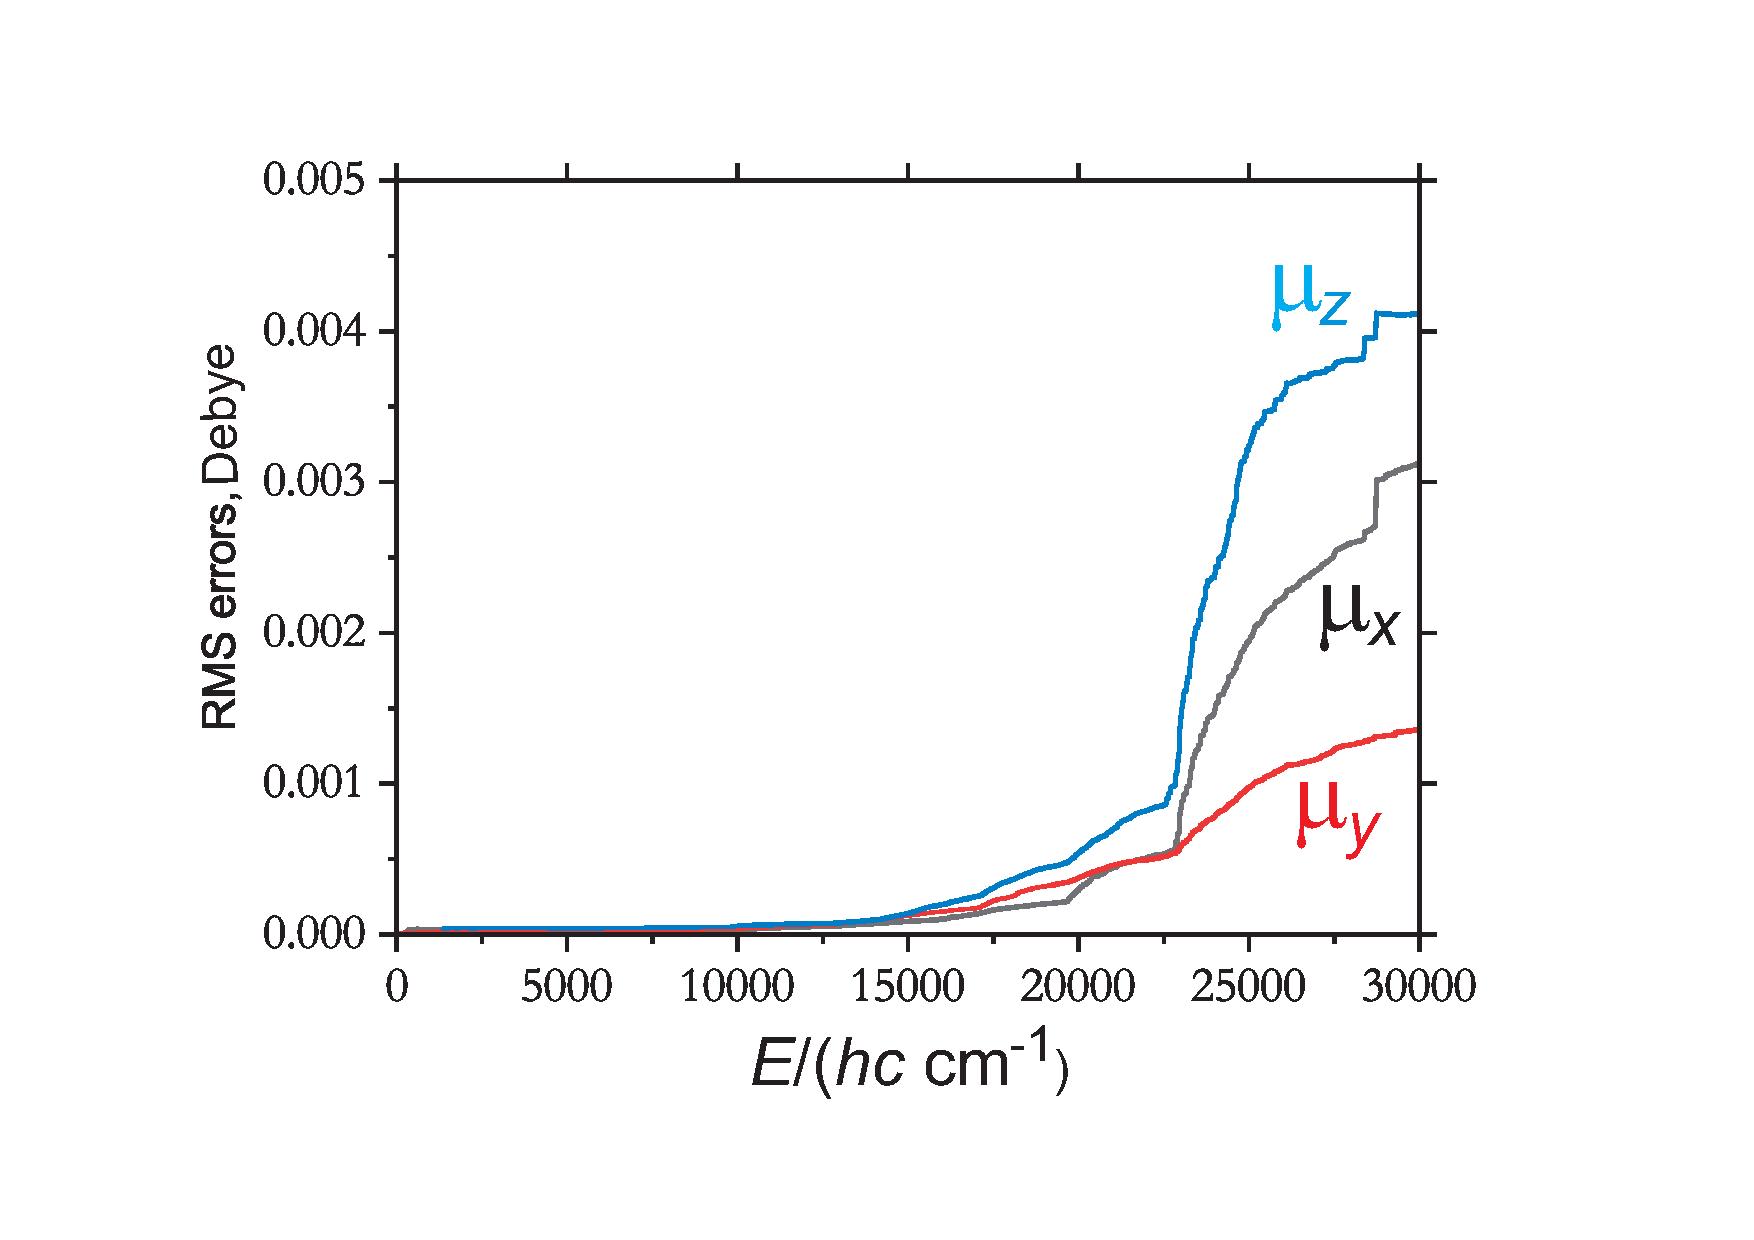
\includegraphics[width=0.9\textwidth]{CH3_RMS_dms.pdf}
\end{center}
\end{figure}

%--------------------------------------------------------------------------
\section{Intensity simulations with TROVE} \label{sec:simulat:range}
%--------------------------------------------------------------------------

%--------------------------------------------------------------
\subsection{General expressions} \label{subs:General-formulas}
%--------------------------------------------------------------

The `readiness' of the molecule to make an absorption or emission transition from an initial ro-vibrational state $i$ to a final ro-vibrational state $f$ is expressed by the  line strength\cite{dipole05,mss,fms}  $S(f\leftarrow i)$, a  quantity with units of [dipole moment]$^2$ (typically Debye$^2$). For $S(f\leftarrow i)$ $=$ 0, the transition does not take place and need not be considered. As discussed in Ref.\citenum{mss} transitions with $S(f\leftarrow i)$ $\ne$ 0 are said to satisfy selection rules which we can derive from symmetry considerations before we do quantitative, numerical calculations of $S(f\leftarrow i)$. Thus, these calculations need only be done for transitions satisfying the selection rules, and after obtaining values of $S(f\leftarrow i)$ for these transitions, we can compute the corresponding  Einstein coefficients
and absorption intensities.

The initial(final) state $i$($f$) has the rotation-vibration wavefunction $\vert \Phi_{\rm rv}^{(i)}
\rangle$($\vert \Phi_{\rm rv}^{(f)} \rangle$).
The line strength\cite{dipole05,mss,fms} $S(f\leftarrow i)$ of the ro-vibrational transition
$f \leftarrow i$ is
%---------
% Equation
%---------
\begin{equation}
\label{e:linestrength_deg}
S(f \leftarrow i) =
g_{\rm ns} \,
\sum_{M_f, M_i} \,
\sum_{A=X,Y,Z}
\left\vert  \left\langle
\Phi_{\rm rv}^{(f)} \,
\left\vert
\bar\mu_A \right\vert
\Phi_{\rm rv}^{(i)}
\right\rangle \right\vert^2 \hbox{,}
\end{equation}
%-------------
where $g_{\rm ns}$ is the nuclear spin statistical weight factor\cite{mss} and $\bar\mu_A$
is the electronically averaged component of the molecular dipole moment along the space-fixed axis\cite{mss}
$A$ $=$ $X$, $Y$, or $Z$. The quantum numbers $M_i$ and $M_f$ are the projections of the total angular
momentum $\hat{\mathbf{J}}$ on the $Z$ axis for the initial and final states, respectively.

Assuming that the molecules considered are in thermal equilibrium at the absolute temperature $T$,
the intensity of a spectral line  is determined as
%---------
% Equation
%---------
\begin{equation}
\label{e:intensity-absorption}
I(f \leftarrow i)  =
    \frac{8 \pi^3 N_A \tilde\nu_{if}}{(4 \pi \epsilon_0)3hc} \,
    \frac{{\rm e}^{-E_i/kT}}{Q} \,
    \big[1 - {\rm exp}(-hc\tilde\nu_{if}/kT)\big] \,
    S(f \leftarrow i).
\end{equation}
%-------------
Here $\tilde{\nu}$ is the absorption wavenumber, and Eq.~\eqref{e:intensity-absorption} refers to the
transition from the state $i$ with energy $E_i$ to the state $f$ with energy $E_f$, where
$hc\tilde\nu_{if}$ = $E_f$$-$$E_i$. $Q$ is the partition function defined as $Q$ $=$ $\sum_j g_j \,
\exp (  -E_j/kT)$, where $g_j$ is the total degeneracy of the state with energy $E_j$ and
the sum runs over all energy levels of the molecule, and other symbols
have their usual meanings. The total degeneracy $g_j$ is given by
$(2J+1)$ times the spin degeneracy ($M = $ 2) and times the nuclear spin degeneracy which is 4, 0, 2, 4, 0, 2
for $A_1\p, A_2\p, E\p, A_1\pp, A_2\pp,$ and $E\pp$ symmetries respectively. The ground electronic
state of CH$_3$ is a doublet  ($\tilde{X}$~$^2A''_2$) with a small splitting\cite{nu2_82c,nu3_97b}
 %\red{Ahmad, can you please provide the splitting}
in the rovibrational energy levels due to spin-rotation interactions, around 0.01 \cm, which we
therefore chose to ignore for this work, byt however scaling the line intensities by the spin-multiplicity factor of 2.

% (see Appendix \ref{AppendixB}).$\epsilon(\tilde{\nu})$-values.

A detailed expression for the line strength of an individual
ro-vibrational transition within an isolated electronic state
of an XY$_3$ pyramidal molecule is given in Eq. (21) of
Yurchenko~\textit{et al.}~\cite{dipole05}.
Provided that the population of the lower (initial) state is
defined by the Boltzmann distribution, we consider only transitions starting from the
levels below $E_{i}^{\rm max}/h c = $ 9\,000~\cm, which
corresponds to  Boltzmann factors of
$\exp(-E_i / k T) > 2\times 10^{-4}$ entering into Eq.~\eqref{e:intensity-absorption} for $T=1500$~K. It is common to use the partition function for estimating the completeness of the line list for a given temperature \cite{jt592}. By considering the ratio $Q_{9000\,{\rm cm}^{-1}}/Q_{\rm total}$, where $Q_{\rm total}$ is the converged partition function value calculated by explicitly summing over all energy levels and $Q_{9000\,{\rm cm}^{-1}}$ is the partition function calculated using only those levels with energies up to the threshold of 9000 \cm. This ratio gives 95~\%\ completeness
at temperatures below 1500 K, which we estimate  as the maximal temperature for our line list. For
similar reasons, the range of the rotational excitations can be
safely limited at $J=40$. The wavenumber range selected is 0 to 10\,000~\cm; the upper energy limit (i.e., the maximal energy for
the final state) corresponds to a term value of $E^{\rm max}/hc $ $=$ 19,000~\cm.

%------------------------------------------------------------------------
\subsection{ Computational details} \label{subs:Computational-details}
%------------------------------------------------------------------------
We use a symmetry-adapted basis set in the variational nuclear motion
calculations. The Hamiltonian matrix is factorized into
size-independent blocks according to the irreducible representations of the {\itshape\bfseries D}$_{3{\rm h}}$(M) molecular symmetry group:\cite{mss} $A_1\p$,
$A_2\p$, $A_1\pp$, $A_2\pp$, $E\p$, and $E\pp $. The
$A_2\p$ and $A_2\pp$ matrices are of no interest for CH\3 as the
corresponding states have zero nuclear spin statistical weights and do not exist in Nature.\cite{mss} % (Appendix \ref{AppendixB}).
The $E\p$ and $E\pp $ matrices each split into two sub-blocks, of which only one must be diagonalized.\cite{mss}

The calculation of the matrix elements
$\langle \Phi_{\rm rv}^{(f)} \, \vert \bar\mu_A \vert \Phi_{\rm
rv}^{(i)} \rangle$ in Eq.~\eqref{e:linestrength_deg} is the
bottle-neck in the spectrum simulations. Here, the wavefunctions $\Phi_{\rm rv}^{(w)} $
are expressed as symmetry-adapted linear combinations of basis functions (see
Eq.~(65) of Yurchenko \textit{et al.}~\cite{trove17a}):
%---------
% Equation
%---------
\begin{equation}
\label{e:rovib:basis}
\vert \Phi_{\rm rv}^{(w)} \rangle =
\sum_{V K \tau_{\rm rot}}
C_{V K \tau_{\rm rot}}^{(w)} \,
\vert J_w \, K \, m_w\, \tau_{\rm rot}  \rangle \, | V \rangle,
\;\; w = i \;\; {\rm or} \;\; f,
\end{equation}
%-------------
where the $C_{V K \tau_{\rm rot}}^{(w)}$ are expansion coefficients,
$\vert J_w \, K \, m_w\, \tau_{\rm rot} \rangle$ is a
symmetrized rotational basis function, $\tau_{\rm rot}$ ($=$ 0
or 1) is associated with the rotational parity, and $\vert V \rangle$ is a vibrational basis function.
In order to speed up this part of the calculations, we applied
a pre-screening procedure to the expansion coefficients $C_{V
K \tau_{\rm rot}}^{(f)}$.
All
terms with coefficients less than the threshold value of
$10^{-13}$ were excluded from the integration.
%\red{Please check! We usually use 1e-12}


A speedup
in the evaluation of the dipole moment
matrix elements $\langle \Phi_{\rm rv}^{(f)} \, \vert \bar\mu_A
\vert \Phi_{\rm rv}^{(i)} \rangle$ can be done
in two steps. First, for a given lower state $i$
the following effective line strength is evaluated:
%---------
% Equation
%---------
\begin{equation}\label{e:effective:Sif}
S_{i,V K}^{A} = \langle \Phi_{\rm rv}^{(i)} \vert \bar\mu_{A} \vert \phi_{V K} \rangle,
\end{equation}
%-------------
where we introduced a short-hand notation $\phi_{V K}$ for the
primitive basis function $\vert J_w K \, m_w\, \tau_{\rm rot}
\rangle$ $\times \vert V \rangle $. Once all $S_{i,V K}$ are computed,
in the second step the line strength $S(f \leftarrow i)$ is
evaluated as
%---------
% Equation
%---------
\begin{equation}\label{e:effective:Sif:2nd:step}
S(f \leftarrow i)= g_{\rm ns} \sum_{m_i, m_f}\sum_{A=X,Y,Z} \left\vert  \sum_{V, K} C_{V K \tau_{\rm rot}}^{(f)} S_{i, V K}^A \right\vert^2.
\end{equation}
%-------------

We had to compute a very large number of transitions satisfying the selection rule
$\vert J_{f} - J_i \vert$ $\leqslant$ 1, where
 $J_{i}$ and $J_f$ are the values of the angular momentum quantum number  $J$ for the initial and final state, respectively. Consequently, we saved memory by organizing the calculation of the ro-vibrational eigenstates and the $S(f\leftarrow i)$-values such that at a given time, only eigenvectors for states with two consecutive $J$-values,  $J$ and $J+1$, are available for the computation of $S(f\leftarrow i)$-values. This algorithm is  implemented in the  GPU GAIN-MPI program \citep{17AlYuTe}.
 



The vibrational basis set $|V\rangle$ is obtained in TROVE using a multi-step contraction and symmetrization procedure, starting from local primitive basis set functions, each depending on one variable only (see Refs.~\citenum{trove07,trove15,trove17a} and references therein).
Thus, a compact representation of the vibrational basis set is obtained in a form
 optimized for the molecule of interest.
 The final vibrational basis set is represented by the eigenfunctions of the purely vibrational part of the Hamiltonian;
we call these eigenfunctions the `$J=0$ basis'.

%-------------------------------------
\section{Results} \label{sec:trove}
%-------------------------------------

%----------------------------------------------------------------------------------------------
\subsection{Basis set convergence and empirical adjustment of the vibrational band centers}
\label{subs:band-centers:adjustment}
%----------------------------------------------------------------------------------------------
The dimensions of the Hamiltonian matrix blocks to be diagonalized
are important in determining
the accuracy with which highly excited ro-vibrational
energies and wavefunctions
 can be
computed, and consequently it is important to derive by
empirical methods the smallest basis set that is consistent
with the required eigenvalue accuracy (that is to say, the
optimum size for `convergence').

TROVE employs polyad number
truncation~\cite{trove05,trove07,trove15} to control the size
of the vibrational basis set, with the polyad number $P$ given by:
%---------
% Equation
%---------
\begin{equation}\label{e:polyad-2}
P =  2 (n_1 + n_2 +n_3) + n_{4} + n_{5} + n_{6},
\end{equation}
%-------------
where $n_i$ are the quantum numbers connected with the primitive
functions $\phi_{n_i}(\xi_i)$. That is, we include in the primitive basis set
 only those functions $\phi_{n_i}(\xi_i)$ for which $P$ $\leq$ $P_{\rm max}$.

The vibrational term values could be converged even more tightly by
extrapolating the energies calculated with different-size basis sets  $P_{\rm max}$
to the complete vibrational basis set limit~\cite{ph3_08}.
However, this is not considered necessary for the purpose of generating
a line list since the corrections from such an extrapolation will be
small compared with the inherent errors in the term values that are
caused by the imperfection of the underlying potential energy surface.
Instead, if we aim for higher accuracy in a pragmatic manner, we can
 resort to a more empirical approach where the theoretical vibrational
term values are replaced by accurate
 experimental  vibrational band centres, whenever these are
available in the literature.
In this case, we adjust the vibrational band centers `by hand', and
by doing so, we shift the rotational energy structure towards better
agreement with experiment.
This procedure can be regarded as an empirical basis set correction
scheme and will be denoted as EBSC scheme.


 We adopt the EBSC scheme for the vibrational bands $2\nu_2$, $\nu_1$, $\nu_4^1$, and $\nu_3^1$, for which accurate experimental data is available, in combination with PES-2, where we have adjusted the equilibrium structure of the molecule to fit the experimentally derived pure rotational term values. The vibrational basis set was truncated at the polyad number $P_{\rm max}=32$.  The incorporation of experimental information in the
EBSC scheme is obviously a departure from a purely \abinitio\ approach
which is considered to be justified by the gain in accuracy that can
be achieved when computing an extensive ro-vibrational line list.

To achieve higher accuracy for
the vibrational band centers, another more thorough refinement of our
PES would be needed. However, considering a severe lack of the accurate experimental data on the vibrationally excited states of CH$_3$, we decided for a pragmatic, alternative procedure based on the EBSC substitution scheme in conjunction with the $r_{\rm e}$-refinement. Even though we cannot avoid imperfections for all bands which where not EBSC-corrected, a more accurate rotational structure should be useful for assignments of future experimental works on CH$_3$.


 \ref{t:energies} lists the vibrational band centers of methyl radical up to 5000~\cm, as derived
from experimental data and from variational calculations of the present work computed using PES 2. 
These experimental band centers were used to replace the theoretical values $P_{\rm max} = 32$ values in all $J>0$ TROVE calculations according with the EBSC substitution. This table also shows the effect of the polyad-number on the
vibrational energy. %Based on the deviations from experiment (before EBSC), we can estimate the \ai\ errors to be within 10~\cm\ with an rms of about 3~\cm\  for term values below 20000 \cm\ \red{sy: I don't really understand where these estimates came from and also not sure if my interpretation of this paragraph was correct, Ahmad please check.}.


%Our own previous refinement that led to PES-1 \red{(AY: PES-2?)} (see above) yielded rms errors of 0.9~\cm\ for the vibrational band centers below 20000 \cm, in variational calculations where the kinetic-energy and  potential-energy expansions were truncated at 6th order and 8th order respectively \red{(AY: the expansion order is not relevant (and hasn't been mentioned before))}. In the  present work, we truncate the potential-energy expansions at 8th order \red{(AY: no need to mention if it is the same)} and use PES-2 (see above). Both these changes will have the effect of ``detuning'' the previous refinement. This can be seen in the  last two columns of \ref{t:energies}  which list the current TROVE  results for PES-2 using $P_{\rm max} = 24$ and $P_{\rm max} = 32$ \red{(AY: not clear what the  reader should look for, that energy unusually increases with increasing the basis set, this is confusing)}. The deviations from experiment are usually in the range of 10 \cm, and the rms errors amount to 1.8 and 2.4~\cm, respectively (for term values below 20000 \cm\  \red{(AY: sorry, the paragraph above is not clear)}).


%----------
% Table 1
%----------

%------------
\begin{table}
%------------
\caption{\label{t:energies}  Vibrational band centers (\cm) of $^{12}$CH\3\ from variational calculations.}
\begin{center}
\tabcolsep=5pt
\renewcommand{\arraystretch}{1.175}
\begin{tabular}{llcr@{}lrrr@{}l}
\hline
\hline
$\Gamma$& State &  Ref. & \multicolumn{2}{c}{Obs.$^a$}   & \multicolumn{1}{c}{$P_{\rm max}=24$$^b$}  & \multicolumn{2}{c}{$P_{\rm max}=32$$^c$} &\\
\hline
$A_1'$  &       $       2\nu_2                  $       & \onlinecite{nu2_81} 	& 1288.1\phantom{00}    &       &       1279.77	&	1281.24	&	\\
        &       $       2\nu_4                  $	& 	                &		        &	&	2737.63	&	2739.64 &	\\
        &	$	4\nu_2	                $	& 	                &	 	        &	&	2773.65	&	2776.86	&	\\
        &	$	 \nu_1	                $	& \onlinecite{nu1_92}   & 3004.42\phantom{0}    &       &       3002.71 &       3002.76 &       \\
        &	$	3\nu_4^3	        $	& 	                &		        &	&	4118.59	&	4120.58	&	\\
        &	$	 \nu_1+2\nu_2	        $	&	                &		        &	&	4258.97	&	4260.53	&	\\
        &	$	6\nu_2	                $	&	                &		        &	&	4391.99	&	4397.00	&	\\
        &	$	 \nu_3^1+\nu_4^1	$	&	                &		        &	&	4537.94	&	4538.93	&	\\
        &       $	4\nu_4	                $	&	                &		        &	&	5371.39	&	5364.56	&	\\
        &       $	2\nu_2+3\nu_4^3	        $	&	                &		        &	&	5475.84	&	5480.07	&	\\
        &	$	4\nu_2+2\nu_4	        $	&	                &		        &	&	5601.91	&	5607.20	&	\\
$ E'$	&	$	 \nu_4^1	        $	& \onlinecite{nu4_94}	& 1397.0\phantom{00}	&	&	1385.99	&	1387.26	&	\\
        &	$	2\nu_2+\nu_4^1	        $	&	                &		        &	&	2688.80	&	2691.61	&	\\
        &	$	2\nu_4^2	        $	&	                &	 	        &	&	2759.77	&	2762.05	&	\\
        &	$	 \nu_3^1	        $	& \onlinecite{nu3_97b}	& 3160.8\phantom{00}	&	&	3158.88	&	3158.83	&	\\
        &	$	3\nu_4^1	        $	&	                &		        &	&	4074.69	&	4075.46	&	\\
        &	$	2\nu_2+2\nu_4^2	        $	&	                &		        &	&	4087.92	&	4091.72	&	\\
$A_2''$	&	$        \nu_2                  $       & \onlinecite{nu1_92}	& 606.453	        &	&	602.43	&	602.43  &	\\
      	&	$       3\nu_2                  $       & 	                & 	                &	&	2010.09	&	2010.09 &	\\
      	&	$        \nu_2+2\nu_4^0         $       & 	                & 	                &	&       3372.27	&	3371.59 &	\\
      	&	$       5\nu_2                  $       & 	                & 	                &	&	3569.96	&	3569.95 &	\\
        &	$        \nu_1+\nu_2            $       & 	                & 	                &	&	3596.35	&	3596.30 &	\\
        &       $       3\nu_4^3                $       & 	                & 	                &	&	4768.70	&	4767.06 &	\\
        &	$        \nu_2+2\nu_4^0         $       & 	                & 	                &	&	4823.32	&	4822.79 &	\\
        &	$        \nu_1+3\nu_2           $       & 	                & 	                &	&	4981.58	&	4981.52 &	\\
$E''$	&	$	 \nu_2+\nu_4^1	        $	&	                &		        &	&	2000.24	&	2002.22	&	\\
        &	$	 \nu_2+2\nu_4^2	        $	&	                &		        &	&	3388.24	&	3391.11	&	\\
        &	$	3\nu_2+\nu_4^1	        $	&	                &		        &	&	3426.45	&	3430.06	&	\\
        &	$	 \nu_2+\nu_3^1	        $	&	                &		        &	&	3736.40	&	3736.97	&	\\
        &	$	 \nu_2+3\nu_4^1	        $	&	                &		        &	&	4726.62	&	4728.62	&	\\
        &	$	3\nu_2+2\nu_4^2	        $	&	                &		        &	&	4835.22	&	4839.85	&	\\
        &	$	 \nu_1+\nu_2+\nu_4^1	$	&	                &		        &	&       4980.92	&	4983.16	&	\\
\hline
\end{tabular}
\end{center}
\begin{flushleft}
\noindent \vspace*{0.1truecm}
$^a$ Experimental values of band centers used to replace the theoretical values $P_{\rm max}=32$, see text.  \\
$^b$ Computed using the $P_{\rm max}=24$ basis set in conjunction with PES-2\cite{aa15}.\\
$^c$ Computed using the $P_{\rm max}=32$ basis set in conjunction with PES-2\cite{aa15}. \\
\end{flushleft}
%----------
\end{table}
%----------


\ref{t:rot:energies} shows a comparison of the pure rotational energies ($J\le 5$) of CH$_3$ before and after refinement of $r_{\rm e}$ illustrating the importance of this step.



%----------
% Table 2
%----------
%------------
\begin{table}
%------------
\caption{\label{t:rot:energies}  Theoretical rotational term
values ($N\le 5$, in \cm) of CH$_3$, computed with TROVE using different
equilibrium structure parameters.}
\begin{center}
\renewcommand{\arraystretch}{0.95}
\begin{tabular}{cccrrrr}
\hline
\hline
\multicolumn{3}{c}{States}  &   \multicolumn{3}{c}{Term values}          \\
\hline
$N$   &  $K$   &$\tau_{\rm rot}$ &  Obs. &  Obs.-Calc.$^a$& Obs.-Calc.$^b$ \\
\hline
1   &   1    &    0    &  14.3189 & 0.032377 &  0.004027 \\
2   &   0    &    1    &  57.4396 & 0.112005 & -0.002023 \\
2   &   2    &    0    &  38.1186 & 0.092340 &  0.017004 \\
2   &   1    &    0    &  52.6112 & 0.106875 &  0.002511 \\
3   &   3    &    0    &  71.3965 & 0.179934 &  0.038989 \\
3   &   2    &    0    &  95.5353 & 0.203902 &  0.014649 \\
3   &   1    &    0    & 110.0032 & 0.219365 &  0.001200 \\
4   &   0    &    0    & 191.2473 & 0.375024 & -0.004034 \\
4   &   4    &    0    & 114.1491 & 0.295456 &  0.070301 \\
4   &   2    &    0    & 172.0038 & 0.353500 &  0.012772 \\
4   &   3    &    0    & 147.9203 & 0.327970 &  0.035289 \\
\hline
\end{tabular}
\end{center}
\begin{flushleft}
\noindent \vspace*{0.1truecm}
$^a$ {Calculated using $r_{\rm e} = 1.07736927$~\AA\ and $\alpha_{\rm e}= 120.0^\circ$ (PES-1, see text).} \\
\noindent \vspace*{0.1truecm}
$^b$ {Calculated using $r_{\rm e} = 1.0762977119$~\AA\ and $\alpha_{\rm e}=120.0^\circ$ (PES-2, see text).}
\end{flushleft}
%----------
\end{table}
%----------




%scheme outlined above which, by construction, will give exact
%agreement with the available experimental band centers in $J=0$
%calculations. When generating a line list using the EBSC scheme, the
%imperfection of the chosen PES will thus enter only through the
%computed band centers of bands where reliable experimental data are
%missing, and through the ro-vibrational couplings that affect the full
%ro-vibrational calculations. Another source of error is the limited
%accuracy of the available experimental data.
%\red{(AY: I suggest to completely skip two paragraphs above)}





%--------------------------------------------------------------------------
%\subsection{Vibrational transition moments} \label{subsec:transmoments}
%--------------------------------------------------------------------------

The vibrational transition moments are defined as
%---------
% Equation
%---------
\begin{equation}\label{e:vib:mu}
 \mu_{V'V} = \sqrt{\sum_{\alpha=x,y,z} | \langle V'\mid \bar\mu_\alpha \mid V \rangle |^2 }
\end{equation}
%-------------
 where $|V'\rangle$ and $|V\rangle$ denote $J=0$ vibrational wavefunctions and $\bar\mu_\alpha$ is the electronically-averaged dipole moment in the molecular frame (see the section entitled `Dipole moment surface' above).
 For calculation of vibrational transition moments we used our \abinitio\ PES-1 and truncated the vibrational basis set at polyad number $P_{\rm max}=32$.
A number of computed transition moments for the strongest lower lying bands are listed in Table 3 where they are compared with the available experimental data
%A number of computed transition moments are listed in \ref{t:tm:1} where they are compared with the available experimental data.
 The complete list of theoretical transition moments is given as Supporting Information and can be also found at \url{www.exomol.com}.

%----------


%-----------
% Table 3
%-----------

%------------
\begin{table}
%------------
\caption{\label{t:tm:1}  Band Centers $\nu_{fi}$ and Vibrational Transition Moments $\mu_{fi}$ for CH$_3$.$^a$}
\begin{center}
\renewcommand{\arraystretch}{1.25}
\begin{tabular}{llllllll}
\hline
\multicolumn{2}{c}{States}       &  \multicolumn{1}{c}{$\nu_{fi}$/\cm} &
\multicolumn{2}{c}{Calc. $\mu_{fi}$/D} & Obs. $\mu_{fi}$/D
   & Ref.    \\
\hline
$f$                            & $i$   \\
\hline
$ 2\nu_2	        $ &   $\nu_2$	 &	678.81	 &	0.25684	  && 0.31(6)   & [\citenum{mu2_08} ] 	           \\
$  \nu_2	        $ &	0        &	602.43	 &	0.20403	  && 0.215(25) & [\citenum{mu2_05,mu2_83,mu2_89} ] \\
$  \nu_3^1	        $ &	0	 &	3158.83	 &	0.03999	  && 0.03(27)  & [\citenum{mu3_95,mu3_94} ] 	   \\
\cline{1-8}
$  \nu_4^1	        $ &	0	 &	1387.26	 &	0.02931	  &&	       &		                   \\
$ 2\nu_3   +  \nu_4	$ &	0	 &	4529.74	 &	0.02049	  &&	       &		                   \\
$  \nu_1   +  \nu_4^1	$ &	0	 &	4383.56	 &	0.00866	  &&	       &		                   \\
$ 2\nu_2   +  \nu_3^1	$ &	0	 &	4396.18	 &	0.00486	  &&	       &		                   \\
$ 2\nu_3^2	        $ &	0	 &	6294.76	 &	0.00462	  &&	       &		                   \\
$  \nu_1   +  \nu_3^1	$ &	0	 &	6076.68	 &	0.00321	  &&	       &		                   \\
$ 2\nu_4^2	        $ &	0	 &	2762.05	 &	0.00313	  &&	       &		                   \\
$  \nu_3^1 + 2\nu_4	$ &	0	 &	5864.94	 &	0.00242	  &&	       &		                   \\
$ 3\nu_4^1	        $ &	0	 &	4075.46	 &	0.00186	  &&	       &		                   \\
$ 2\nu_2+\nu_3^1+\nu_4^1$ &	0	 &	5789.16	 &	0.00130	  &&	       &		                   \\
$ 4\nu_2	        $ &	0	 &	5856.39	 &	0.00116	  &&	       &		                   \\
\hline
\end{tabular}
\end{center}
\begin{flushleft}
\noindent \vspace*{0.1truecm}
$^a$ The transitions originate in the vibrational ground state
($i=0$) with the exception of the hot band $2\nu_2\leftarrow\nu_2$.
\end{flushleft}
%----------
\end{table}
%----------


%-------------------------------------------------
\subsection{Intensity simulations} \label{subsec:intens}
%-----------------------------------------------------------
In order to simulate absorption spectra at a given temperature $T$ and within a
particular wavenumber range, the upper and lower energies and the
Einstein coefficients $A(f \leftarrow i)$ [or the line strengths
$S(f \leftarrow i)$; the relationship between
 $A(f \leftarrow i)$ and
$S(f \leftarrow i)$ is described in Ref.~\citenum{dipole05}] of
all transitions in this range must be known; in practice, only the
transitions above a certain minimum intensity are included. The
simplest way to present the spectral data is a `stick' diagram
where the height gives the integrated absorption coefficient from
Eq.~\eqref{e:intensity-absorption}. In this section we report such
simulations for the CH$_3$ absorption bands covering the frequency
range 600--1200~\cm\ for the out-of-plane bending mode $\nu_2$. The line strengths in
Eq.~\eqref{e:intensity-absorption} are computed from
Eq.~\eqref{e:linestrength_deg} with the spin statistical weights
$g_{\rm ns}$ from Ref.~\citenum{aa15}.
The simulations are carried out using PES-2 and the computed DMS
described above.
We used a partition-function value of $Q$ $=$ 732.734,
obtained at 300~K by summing over all variational term values ($J\le 40$) below
36871.73~\cm. With the limits defined above, we computed
2,058,655,166 transitions using the GPU GAIN-MPI program.\citep{17AlYuTe}

\ref{fig:overview} gives an overview (log-scale) of the absorption spectrum of CH$_3$ at different temperatures produced using the line list (log-scale) by means of the ExoCross program\cite{exocross}. \ref{fig:296K} shows  four regions with the strongest, dipole-allowed bands $\nu_2$, $\nu_4$, $\nu_3$ and $\nu_3+\nu_4$.


\begin{figure}[h]
\begin{center}
\caption{\label{fig:overview} An overview of the absorption spectrum (cross sections) of CH$_3$ at different temperatures $T=$ 300, 500, 1000 and 1500~K generated using our line list and the Gaussian line profile with the full-width-at-half-maximum of 1~\cm.    }
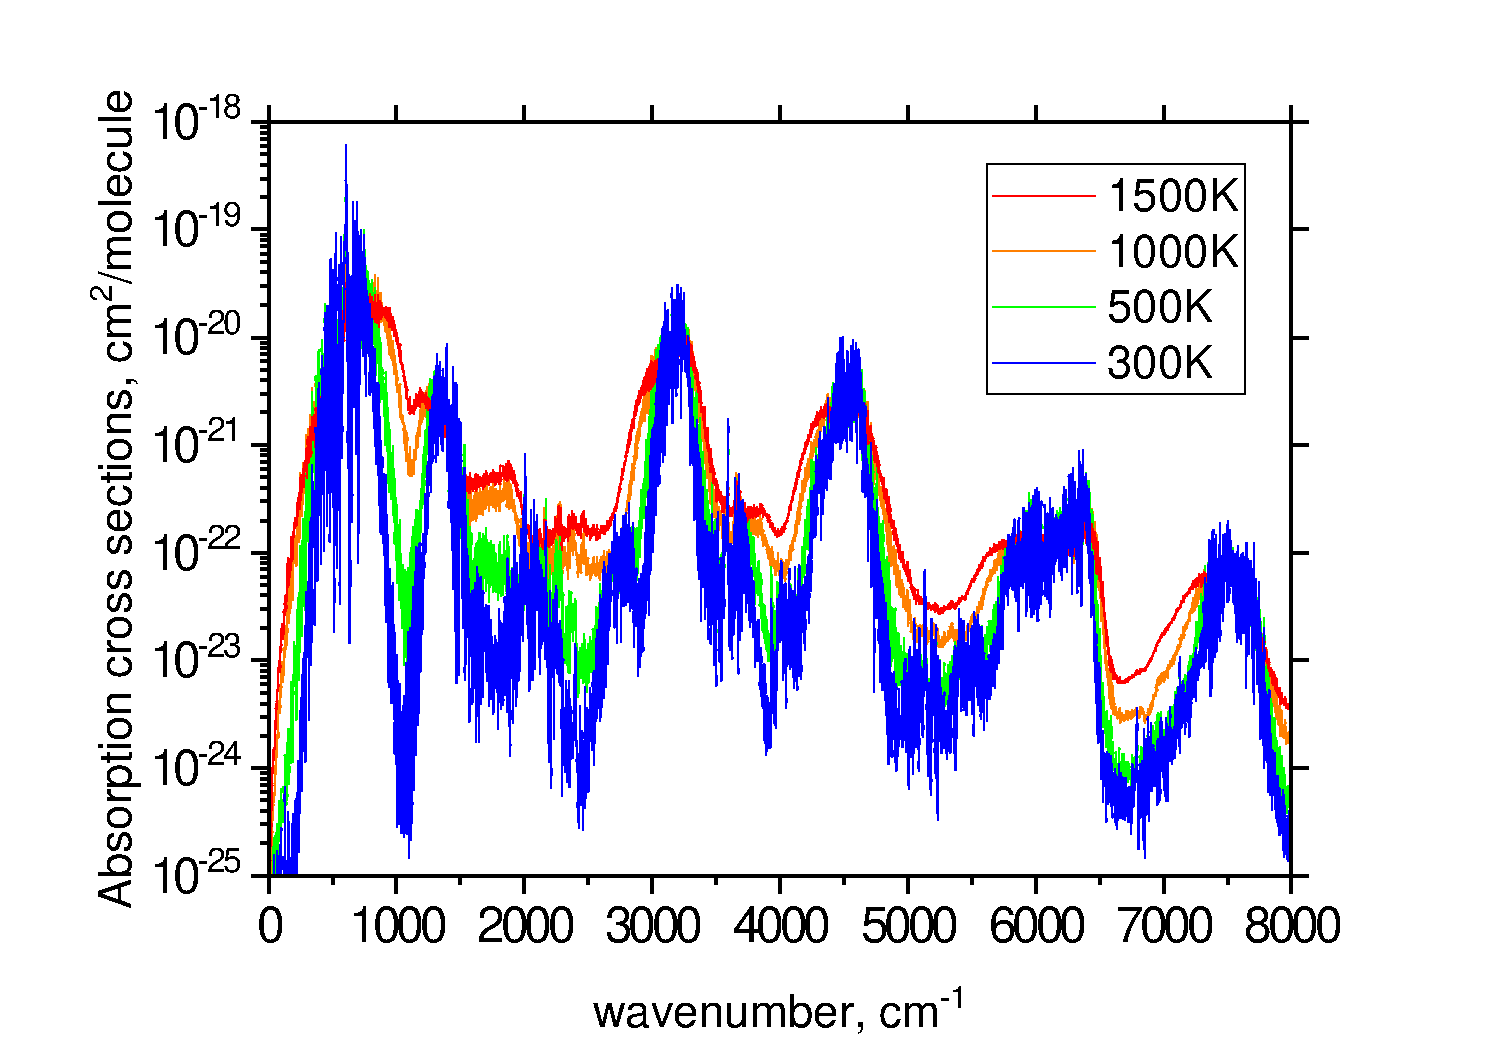
\includegraphics[width=0.9\textwidth]{CH3_T.pdf}
\end{center}
\end{figure}



\begin{figure}[h]
\begin{center}
\caption{\label{fig:296K} A selection of the strongest absorption bands of CH$_3$ at $T=296$~K generated using the line list.  A Gaussian line profile with the half-width-half-maximum of 0.08~\cm\ was used in production of the cross sections shown.  }
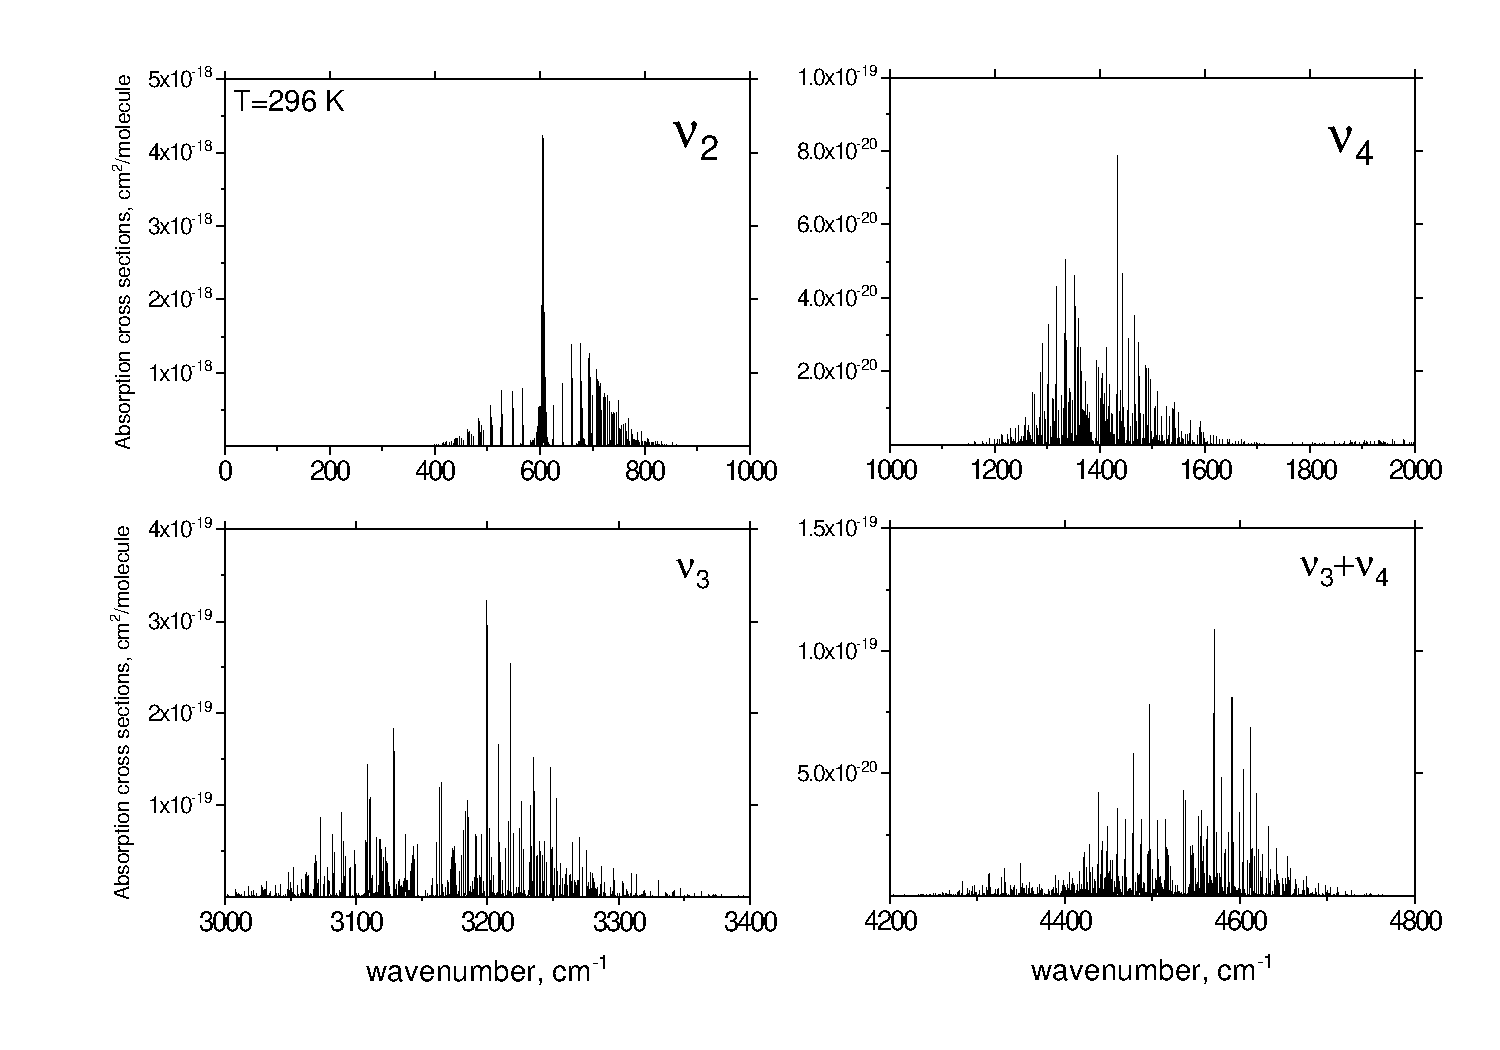
\includegraphics[width=0.9\textwidth]{CH3_4bands.pdf}
\end{center}
\end{figure}

\ref{fig:nu2} shows the emission spectrum of CH$_3$ in
the wavenumber interval 600-1200~\cm,
simulated with TROVE
at two different levels of theory,
rovibrational and purely vibrational. The simulated spectra are compared to
an experimental spectrum recorded by
Hermann and Leone\cite{nu2_82a,nu2_82b} (see Fig.~4 of Ref.~\citenum{nu2_82a}).



\begin{figure}[h]
\begin{center}
\caption{\protect\label{fig:nu2}
Emission spectra of CH\3.
(a)
Rovibrational simulation assuming the CH$_3$ radicals to be in
thermal equilibrium at
 $T$ $=$ 300~K.
(b)
CH$_3$ ($\nu_2$) out-of-plane bending mode
emission spectrum (dots) obtained\protect\cite{nu2_82a}
after
 dissociation of
CH$_3$I $\rightarrow$ CH$_3$($\nu_2$) + I$^*$.
  The continuous curve is the best fit\protect\cite{nu2_82a}
 involving the hot bands
 $(v_2+1)\, \nu_2$ $\leftarrow$
 $v_2\, \nu_2$ with
 $v_2$ $\leqslant$ 9. The spectrum is
convolved with a
 spectrometer slit function with a FWHM of
33~\cm\ and a 19~\cm\ bandwidth ascribed to the breadth of the $\Delta K$ $=$ 0 manifold of transitions with varying $J$ values.
Reproduced from
Ref.~\citenum{nu2_82a}
 with the permission of AIP Publishing.
(c)
Vibrational simulations
at temperatures $T$ $=$ 1000, 2000, and 3000~K, respectively, taking into account the vibrational
transitions
 $(v_2+1)\, \nu_2$ $\leftarrow$
 $v_2\, \nu_2$ with
 $v_2$ $\leqslant$ 9 (see text).
}
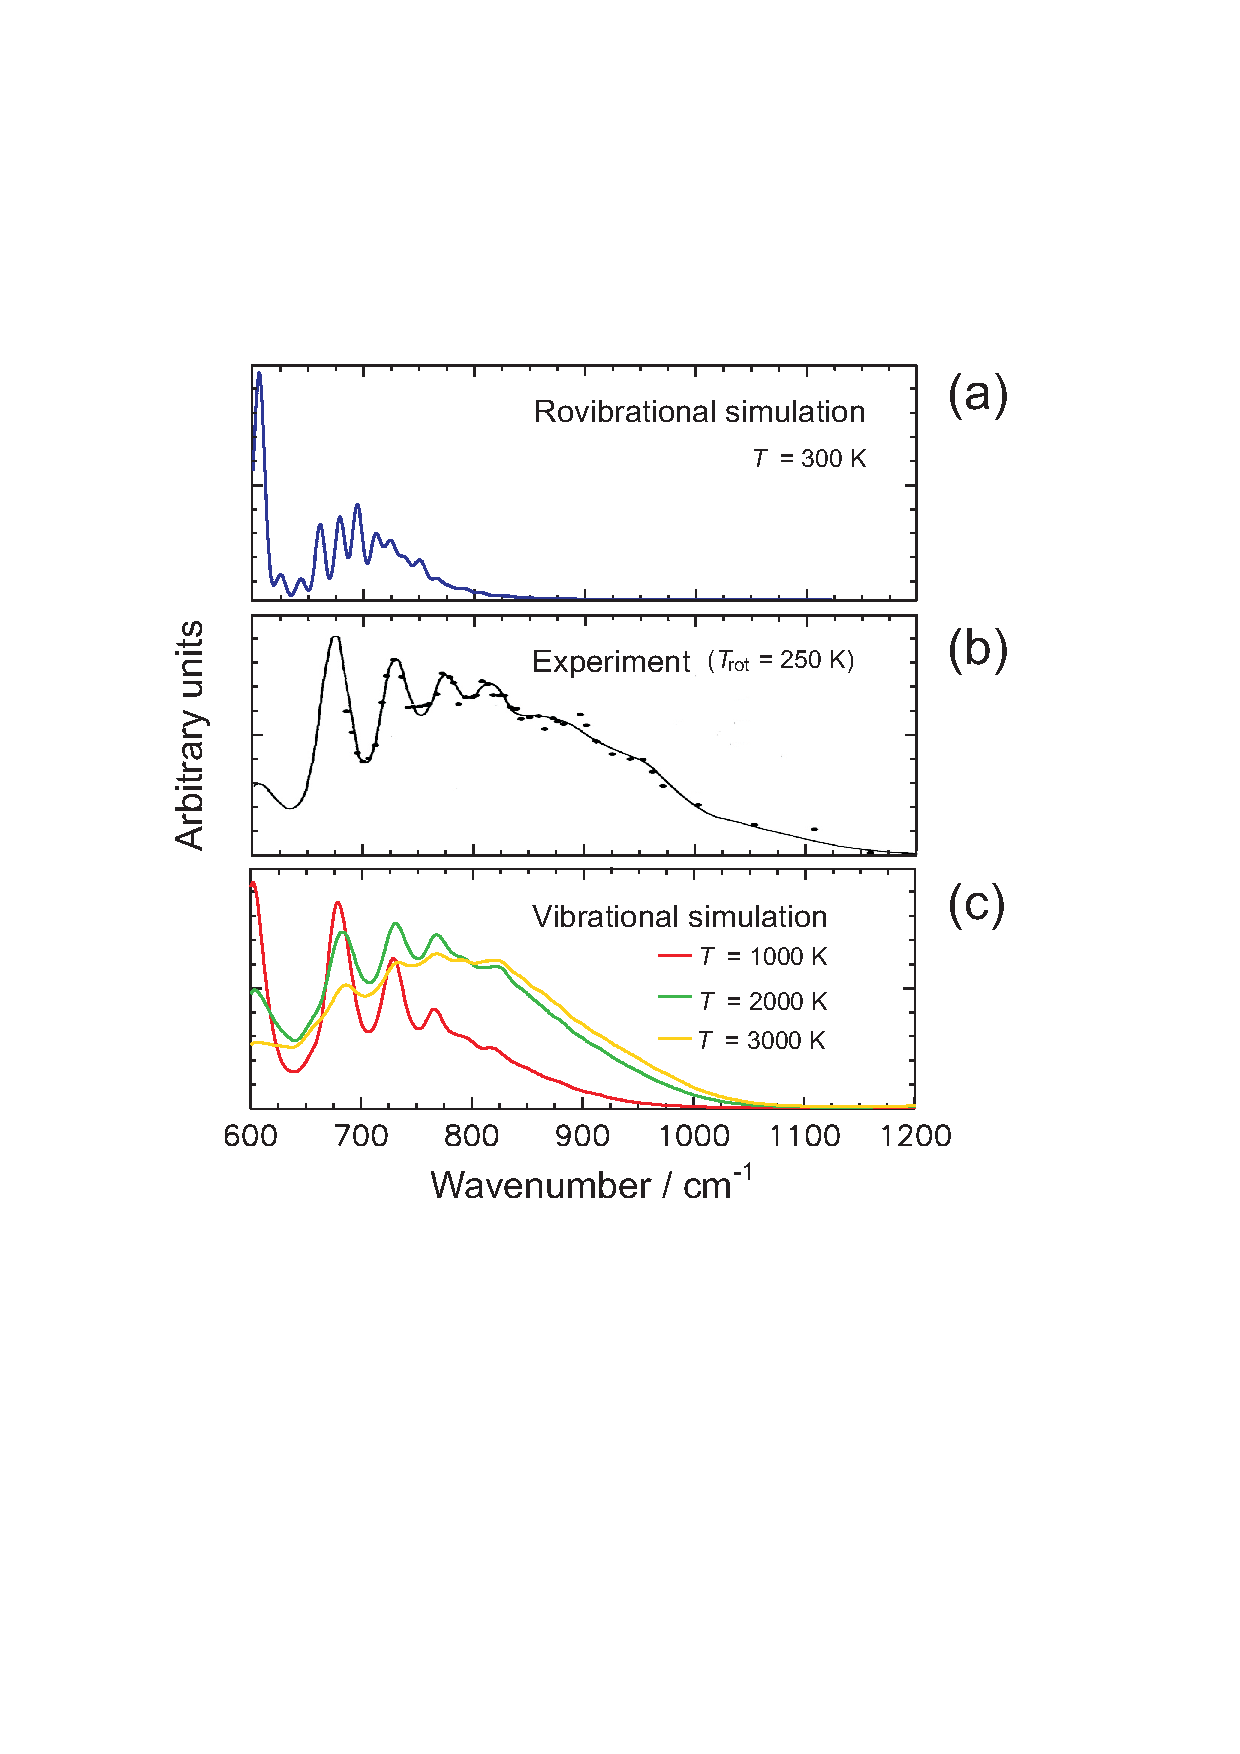
\includegraphics[width=0.8\textwidth]{CH3_LinLis_Fig1.pdf}
\end{center}
\end{figure}


\ref{fig:nu2}(a)  shows a simulation of the CH$_3$ emission spectrum, computed with
TROVE at a temperature of $T$ $=$ 300~K, taking into account all vibrational transitions
in the 600-1200~\cm\ interval that are calculated with the $P_{\rm max} = 32$ basis set. The simulation involves the convolution of the calculated intensities with a Gaussian line shape function with a full width at half maximum (FWHM) of 17~cm$^{-1}$.

The simulation is compared with the experimental spectrum obtained by
Hermann and Leone\cite{nu2_82a,nu2_82b}, shown in
\ref{fig:nu2}(b).\footnote{Reproduced from
Hermann, H. W.; Leone, S. R. The Journal of Chemical Physics 1982, 76, 4759--4765,
 with the permission of AIP Publishing.}
 In the experiment, the CH$_3$ radicals
were
produced the in a photo-fragmentation process
of methyl iodide CH$_3$I.
Hermann and Leone\cite{nu2_82a,nu2_82b} suggested that after the breaking of the C--I bond,
 the CH$_3$ radicals are predominantly produced in excited states of the out-of-plane bending mode
 $\nu_2$. The CH$_3$ fragment of a dissociated CH$_3$I molecule will typically have a pyramidal structure close
to that of the methyl group in
  CH$_3$I. For a CH$_3$ radical, however, which is planar at equilibrium, such structures are associated with
high excitations of the $\nu_2$ vibrational mode.
 Excitations with $v_2$ $\leqslant$  10 have been
observed in the
emission experiment
of Refs.~\citenum{nu2_82a,nu2_82b}.


In order to simulate vibrationally very hot transitions (hotter than 1500~K) corresponding to
the experimental spectrum of
Refs.~\citenum{nu2_82a} which involves out-of-plane bending states
 $v_2\, \nu_2$ with $v_2$ $\leqslant$  10, we have carried out simulations employing
a so-called one-band model (with the one band being the $\nu_2$ fundamental band here). In the one-band
model, we use the $\nu_2$-band data from the
`parent',
 300~K
 ro-vibrational line list also for the hot bands accompanying the
 $\nu_2$ band. The procedure employed is detailed in
 Ref.~\citenum{jt729} and we outline it briefly here:
We initially produce the
 300~K, $\nu_2$-band cross sections by means of the ExoCross program\cite{exocross} and convolve them
with a Gaussian profile of   FWHM $=$ 17~cm$^{-1}$ between 0 and 1200~cm$^{-1}$, generating 1201 data points. Then the
wavenumbers of the computed cross sections are shifted by
$-$606.4531~cm$^{-1}$, positioning the band center at zero, and the cross sections are normalized.
 A local version of ExoCross now obtains,
 from             the vibrational transition moments computed with TROVE,
the vibrational band intensities
for the hot bands
 $(v_2+1)\, \nu_2$ $\leftarrow$
 $v_2\, \nu_2$,
 $v_2$ $\leqslant$ 9. Finally, the simulated spectrum is generated  by placing,
for each hot band,
 the $\nu_2$-band profile
at the band center $\nu_{fi}$ of the hot band in question, scaled by its
vibrational band intensity.
Such simulations have been carried out for
 temperatures $T$ of  1000, 2000, and 3000~K, respectively, and the results are shown in
\ref{fig:nu2}(c),
   where they can be compared to the experimental results\cite{nu2_82a,nu2_82b}
in
\ref{fig:nu2}(b).


\ref{fig:nu2}(c)   shows that the `standard'
 $T$~$=$~300~K rovibrational simulation of the CH$_3$ emission spectrum
[\ref{fig:nu2}(a)]
has little resemblance to
the experimental spectrum from
  Ref.~\citenum{nu2_82a}
[\ref{fig:nu2}(b)]. Obviously in the experiment, the CH$_3$ molecules populate states
of much higher energies than those accessed in thermal equilibrium at
 $T$~$=$~300~K. However, among the `vibrational simulations' in
\ref{fig:nu2}(c), the curve obtained for
 $T$~$=$~2000~K has a very substantial similarity to the experimental curve. This confirms the
suggestion by
Hermann and Leone\cite{nu2_82a,nu2_82b} that dissociation of
 CH$_3$I  produces
 CH$_3$ radicals in highly excited states of the out-of-plane bending mode $\nu_2$.
The successful simulation of the emission spectrum of
Refs.~\citenum{nu2_82a,nu2_82b} lends credibility to the
 \abinitio\ DMS of the present work; the
intensities based on
this DMS are in very good qualitative agreement with experiment.

Our complete $T=1500$~K CH$_3$ line list is accessed via the repository  \url{www.zenodo.org}, see Ref.~\citenum{19AdYaYu.zenodo}.
%\red{sy: I trust Ahmad will have all Supporting Information files prepared: line list and fortran programs as well as a readme file (thanks!). I don't know if the line list won't be too large for that. We could host the line list at ExoMol and supply the subroutines only}.
It details the transition energies, line strengths, Einstein
coefficients $A(f \leftarrow i)$ and the temperature dependent partition function $Q(T)$. The line list should be applicable for the temperatures below 1500~K. However, the simulated spectra will become increasingly inaccurate with increasing temperature. The line list is given using the ExoMol format\cite{exomol} which can be used together with the ExoCross program\cite{exocross} to generate spectra of CH$_3$.

%----------------------
\section{Conclusion}
%----------------------

We have presented calculated spectra for the methyl radical covering a large
part of the infrared region.
Detailed comparisons with observed room-temperature spectra show
excellent agreement for the position and intensity of the transitions.

Our ultimate aim is the construction of a CH$_{3}$ line list capable
of reproducing and predicting observed spectra at temperatures much higher than  300~K.
This will facilitate
 detections of the methyl radical in space.
The work presented here represents the first step towards this goal, which
involves the generation, refinement, and validation of the required
potential energy and dipole moment surfaces, as well as establishing
the level of accuracy that can be achieved in the variational nuclear-motion
calculations with our computational resources.
In this initial phase, we have produced an methyl radical line list consisting
of 2 billion transitions between 9,127,123 energy levels for ro-vibrational
states up to $J_{\rm max}$ = 40 and energies up to 19~000~cm$^{-1}$.
%Even though this list is less complete and less accurate than ultimately desired,
%it can be used to produce simulated CH$_3$ spectra that
%agree well with observation at room temperature.

\clearpage

%----------------------
\begin{acknowledgement}
%----------------------
A.Y. acknowledges support from DESY (HGF IVF) and from the Cluster of Excellence 'The Hamburg Centre for Ultrafast Imaging' of the Deutsche Forschungsgemeinschaft (DFG) - EXC 1074 - project ID 194651731.
S.Y. is grateful for support from the UK Science and Technology Research Council (STFC)
ST/R000476/1. This work made extensive use of UCL's Legion high performance (HPC) computing facilities as well as of HPC provided by DiRAC supported by STFC and BIS.
It was further supported in part by  grant JE 144/25-1 from the DFG.
%--------------------
\end{acknowledgement}
%-------------------

%---------------
\begin{suppinfo}
%---------------
The Supporting Information for this work includes: (i) dipole moment parameters $\mu_{k,l,m,\ldots}^{(\Gamma)}$,  (ii) potential energy parameters
$f_{jk\dots}^{(s)}$; (iii) Fortran routines for calculating the dipole moment and potential energy values for a given geometry.  Our complete $T=1500$K CH$_3$ line list together with the partition function can be accessed via the Zenodo repository, \url{www.zenodo.org}~\cite{19AdYaYu.zenodo} as well as at \url{www.exomol.com}.


%-------------
\end{suppinfo}
%-------------

\clearpage

%----------
% Table 1
%----------


\clearpage


%-----------------
\clearpage
\begin{center}
FIGURE CAPTIONS
\end{center}
%-----------------

\begin{list}{}{\leftmargin 2cm \labelwidth 1.5cm \labelsep 0.5cm}
\item[\ref{fig:rms-DMS}]
Root-mean-square (RMS) errors of the fittings to the \ai\ dipole moment values.
The results of a series of fittings are shown. In each fitting, the data set includes the \ai\ points with
electronic energy (relative to the potential energy minimum) $V$ $\leqslant$ $E$ (see text).
\item[\ref{fig:overview}]  An overview of the absorption spectrum (cross sections) of CH$_3$ at different temperatures $T=$ 300, 500, 1000 and 1500~K generated using our line list and the Gaussian line profile with the full-width-at-half-maximum of 1~\cm..
\item[\ref{fig:296K}] A selection of the strongest absorption bands of CH$_3$ at $T=296$~K generated using the line list.  A Gaussian line profile with the half-width-half-maximum of 0.08~\cm\ was used in production of the cross sections shown.
\item[\ref{fig:nu2}]
Emission spectra of CH\3.
(a)
Rovibrational simulation assuming the CH$_3$ radicals to be in
thermal equilibrium at
 $T$ $=$ 300~K.
(b)
CH$_3$ ($\nu_2$) out-of-plane bending mode
emission spectrum (dots) obtained\protect\cite{nu2_82a}
after
 dissociation of
CH$_3$I $\rightarrow$ CH$_3$($\nu_2$) + I$^*$.
  The continuous curve is the best fit\protect\cite{nu2_82a}
 involving the hot bands
 $(v_2+1)\, \nu_2$ $\leftarrow$
 $v_2\, \nu_2$ with
 $v_2$ $\leqslant$ 9. The spectrum is
convolved with a
 spectrometer slit function with a FWHM of
33~\cm\ and a 19~\cm\ bandwidth ascribed to the breadth of the $\Delta K$ $=$ 0 manifold of transitions with varying $J$ values.
Reproduced from Fig.~4 of
Ref.~\citenum{nu2_82a}
 with the permission of AIP Publishing.
(c)
Vibrational simulations
at temperatures $T$ $=$ 1000, 2000, and 3000~K, respectively, taking into account the vibrational
transitions
 $(v_2+1)\, \nu_2$ $\leftarrow$
 $v_2\, \nu_2$ with
 $v_2$ $\leqslant$ 9 (see text).
\end{list}


%----------------

\clearpage

%-------
% Figure
%-------

\clearpage

%-----
% bib
%-----

\bibliography{ch3_ir}

%-------------
\end{document}
%-------------
